% --------------- PLANTILLA MAXI (GOD) -----------------
\documentclass[11pt, twocolumn]{article}

\usepackage[latin1,utf8]{inputenc}
\usepackage{verbatim}
\usepackage{multirow}
\usepackage{float}
\usepackage{enumerate}
\usepackage{graphics,graphicx,xcolor}
\usepackage{subfig}
\usepackage[spanish,es-tabla]{babel}
\usepackage{caption}
\usepackage{placeins}
\usepackage{afterpage}
\usepackage{blindtext}
\usepackage{multicol}
\usepackage{geometry}
\usepackage{lipsum}

%paquete para referencias
\usepackage[backend=biber, style=nature, citestyle=numeric, sorting=none, maxbibnames=99]{biblatex} % 
% \usepackage{natbib}
% \bibliographystyle{apsrev4-1} % Utiliza el archivo .bst de APS o uno similar

\usepackage{titling} % Paquete para personalizar título del documento
\usepackage{authblk}  % Paquete para personalizar autores del documento
\renewcommand\Authand{ y } % Reemplazar 'and' con 'y'

\DeclareCaptionFormat{custom}
{%
    \textbf{#1#2}\textit{\small #3}
}
\captionsetup{format=custom}

\newgeometry{bottom=3cm, top=2cm, left=3cm, right=3cm}
\usepackage{hyperref}
\hypersetup{
  colorlinks   = true, %Colours links instead of ugly boxes
  urlcolor     = blue, %Colour for external hyperlinks
  linkcolor    = black, %Colour of internal links
  citecolor   = black %Colour of citations
}

%paquete para unidades
\usepackage{siunitx}
% seteo punto como separador decimal
\AtBeginDocument{\decimalpoint}


% \DeclareSIUnit\torr{Torr}

%% Paquetes de la AMS
\usepackage{amsmath, amsthm, amsfonts, amssymb}

%componentes de texto
\usepackage{textcomp}


% Personaliza título del documento
\pretitle{\begin{center}\LARGE\bfseries}
    \posttitle{\par\vspace{0.5em}\end{center}\large}
    \preauthor{\begin{center}\large \lineskip 0.8em \begin{tabular}[t]{c}}
    \postauthor{\end{tabular}\par\end{center}}
    \predate{\begin{center}\large}
    \postdate{\par\end{center}}


\usepackage{fancyhdr}
\pagestyle{fancy}

% Definimos el encabezado de las paginas pares e impares.
\lhead{REDES NEURONALES}
\chead{Práctica 5 - 2024}
\rhead{Gatto Maximiliano}
\renewcommand{\headrulewidth}{0.5pt}

% aqui definimos el pie de pagina de las paginas pares e impares.
\lfoot[a1]{}
\cfoot[c1]{\thepage}
\rfoot[e1]{}

\renewcommand{\footrulewidth}{0.5pt}

% ------------------- TITULO ----------------------
\title{{\large REDES NEURONALES - PRÁCTICA 5 - 2024} \\ \vspace{1cm}\textbf{Aprendizaje no supervisado}}



\author[ ]{\textbf{Maximiliano Gatto}}
\affil[ ]{Instituto Balseiro (UNCuyo - CNEA) - Bariloche, Río Negro, Argentina\vspace{0.4cm}}
\affil[ ]{\href{mailto:maximiliano.gatto@ib.edu.ar}{maximiliano.gatto@ib.edu.ar}}

\date{\today}

\begin{document}
\maketitle

% ------------------ INTRODUCCION ---------------------
\section{Introducción}

En esta práctica se analizaron diferentes técnicas de aprendizaje no supervisado. En particular, se implementó la regla de hoja y el ``future mapping''. Se verificó el funcionamiento de los algoritmos y se analizaron las convergencias comparando con los resultados obtenidos en las clases teóricas. Todos los ejercicios fueron implementados mediante un script en \texttt{Python}, cuyo código está disponible en este \href{https://github.com/elmasi2393/Redes-neuronales/tree/main}{enlace}.


% ------------------ RESULTADOS ---------------------
\section{Resultados}

% --------------- EJERCICIO 1 ---------------------
\subsection*{Ejercicio 1}
Se considera una red de una capa lineal, con 4 entradas y 1 salida, en donde la salida de la red está dada por \(V = \sum_{j=1}^4 \omega_J X_j\), donde \(X_j\) son las entradas y \(\omega_j\) son los pesos sinápticos. 

La distribución de probabilidad de los valores de entrada de corresponden con una distribución gaussiana multidimensional con media 0 dada por

\begin{equation} \nonumber
    P(X) = \frac{1}{(2\pi)^{2}|\Sigma|^{1/2}} \exp \left( -\frac{1}{2} \overline{X}^T \Sigma^{-1} \overline{X} \right),
\end{equation}

cuya matriz de covarianza es

\begin{equation} \nonumber
    \Sigma = \begin{pmatrix}
        2 & 1 & 1 & 1 \\
        1 & 2 & 1 & 1 \\
        1 & 1 & 2 & 1 \\
        1 & 1 & 1 & 2 \
    \end{pmatrix}.
\end{equation}
\\ 

Se utilizaron valores aleatorios pequeños \([-0.01, 0.01]\) distribuidos uniformemente como condición inicial para los pesos \(\omega\), y se los modificó según la regla de oja analizada en la clase teórica

\begin{equation} \nonumber
    \Delta \omega_{i,j} = \eta V (X_i - V \omega_j), 
\end{equation}

\noindent donde se utilizó arbitrariamente una taza de aprendizaje \(\eta = 0.005\).

Según lo estudiado en la clase teórica, siguiendo la regla de oja, los pesos obtenidos luego del aprendizaje convergen en media al autovector normalizado correspondiente al autovalor más grande de la matriz de covarianza \(\Sigma\). En este caso, el autovector correspondiente al autovalor más grande de \(\Sigma\) es \(\overline{\chi}_{\Sigma} = [0.5, 0.5, 0.5, 0.5]\). 

% \begin{equation} \nonumber
%     \chi_{\Sigma} = \begin{pmatrix}
%         0.5 \\
%         0.5 \\
%         0.5 \\
%         0.5
%     \end{pmatrix}.
% \end{equation}
% \(\overline{\chi}_{\Sigma} = [0.5, 0.5, 0.5, 0.5]\). 

Se utilizaron \(10^7\) ejemplos obtenidos de la distribución gaussiana multidimensional. Los resultados obtenidos para los pesos según el número de ejemplos o épocas del proceso de aprendizaje se muestran en la Figura \ref{fig:ej1_pesos}.

\begin{figure*} [t]
    \centering
    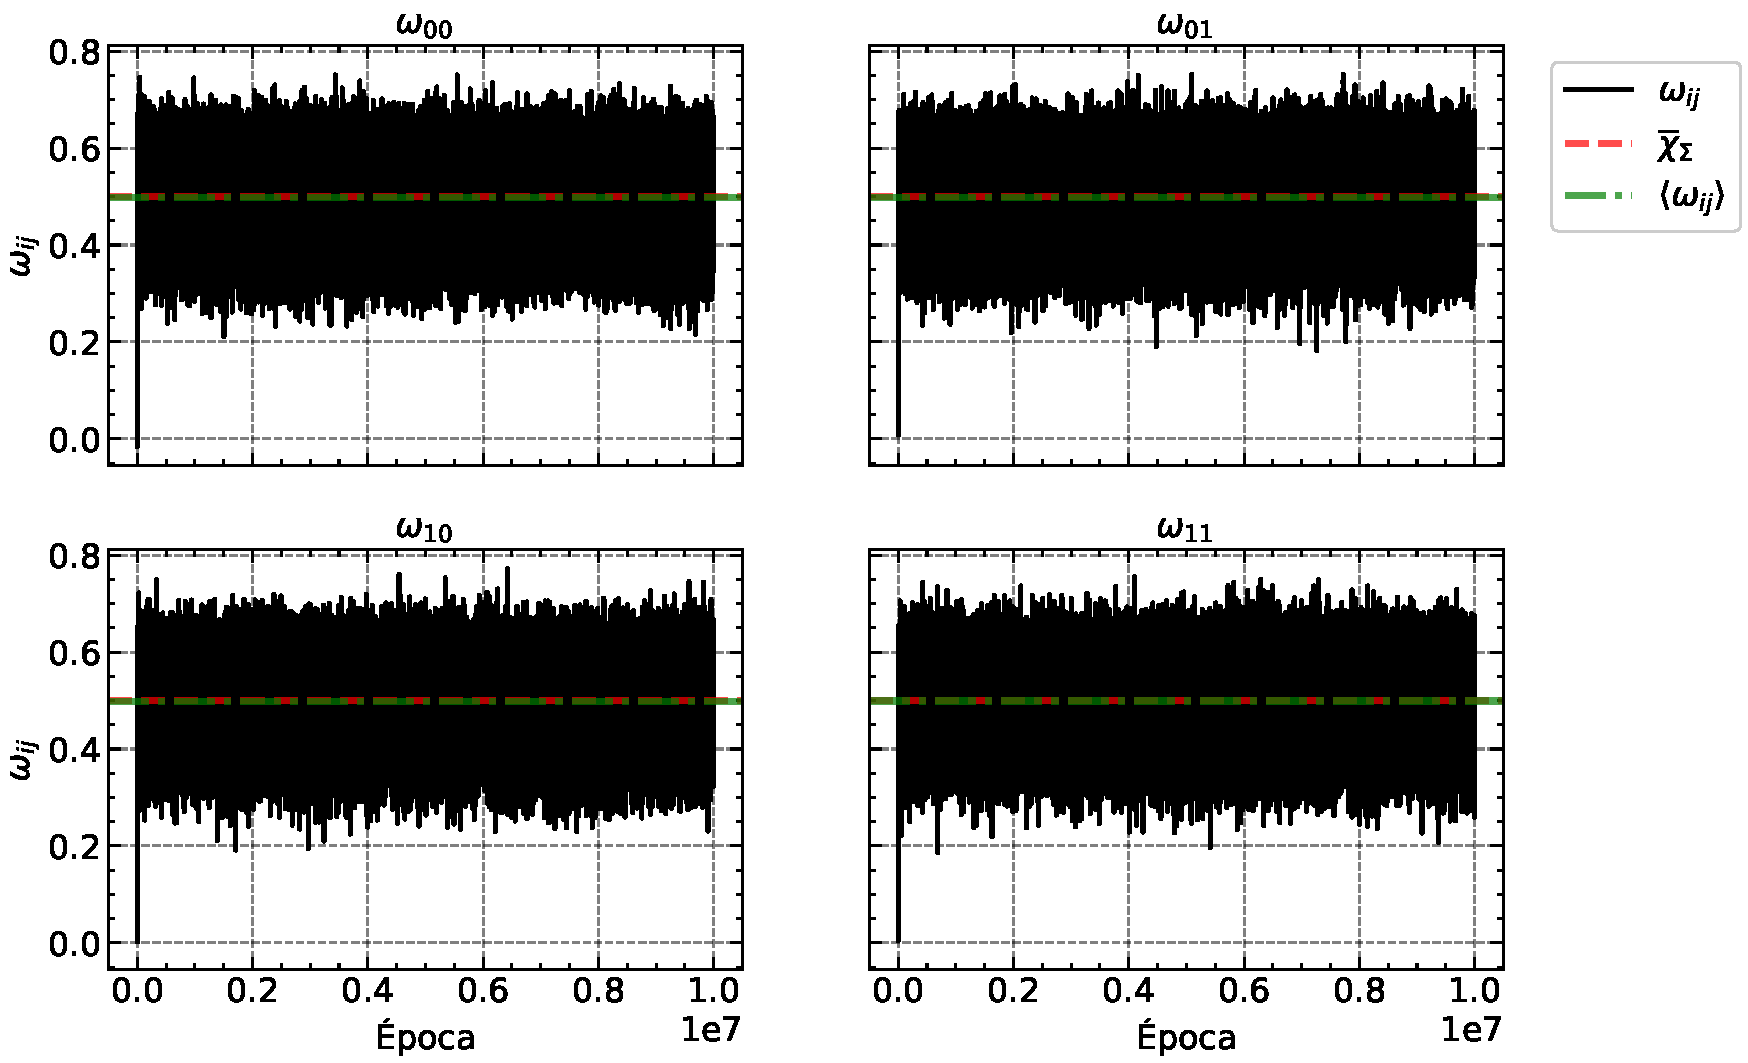
\includegraphics[width=\textwidth]{figures/ej_1.pdf}
    \caption{evolución de los pesos sinápticos durante el proceso de aprendizaje. La línea negra representa el valor de cada una de las componentes de los pesos, la línea de trazos roja representa el valor del autovector en cada componente y la linea de trazo y punto verde representa el valor medio del peso. Se observa que el valor de los pesos es ruidoso, sin embargo el promedio de los pesos converge al autovector de mayor autovalor.}
    \label{fig:ej1_pesos}
\end{figure*}

% --------------- EJERCICIO 2 ---------------------
\subsection*{Ejercicio 2}
Se consideró una red neuronal de Kohonen para analizar la técnica de \textit{feature mapping}, en donde en lugar de solo modificar la unidad ganadora, también se modifican los vecinos. En este ejercicio, se utilizaron 2 neuronas de entradas y 10 neuronas de salidas dispuestas sobre una línea. 

Los datos de entrada de la red se extrajeron de una distribución de probabilidad dada por

\begin{equation} \nonumber
    P(\overline{\xi}) = P(r, \theta) =  
    \begin{cases}
        C \, \, \text{si } r \in [0.9, 1.1], \theta \in [0, \pi] \\
        0 \, \, \text{sino}
    \end{cases}
\end{equation}

\noindent donde \(C\) es una constante de proporción.

Notar que este dominio se corresponde con un ``semi anillo'', en donde la probabilidad es uniforme. Para obtener datos con distribución uniforme en este dominio, se generaron datos en coordenadas cartesianas \((x,y)\) con distribución uniforme en \(x \in [-1.1, 1.1]\) e \(y \in [0, 1.1]\), y se descartaron aquellos puntos que no se encontraban en el semi anillo. Los valores \(\omega_j\) utilizados como condición inicial se muestran en la Figura \ref{fig:cond_inicial}.

\begin{figure}
    \centering
    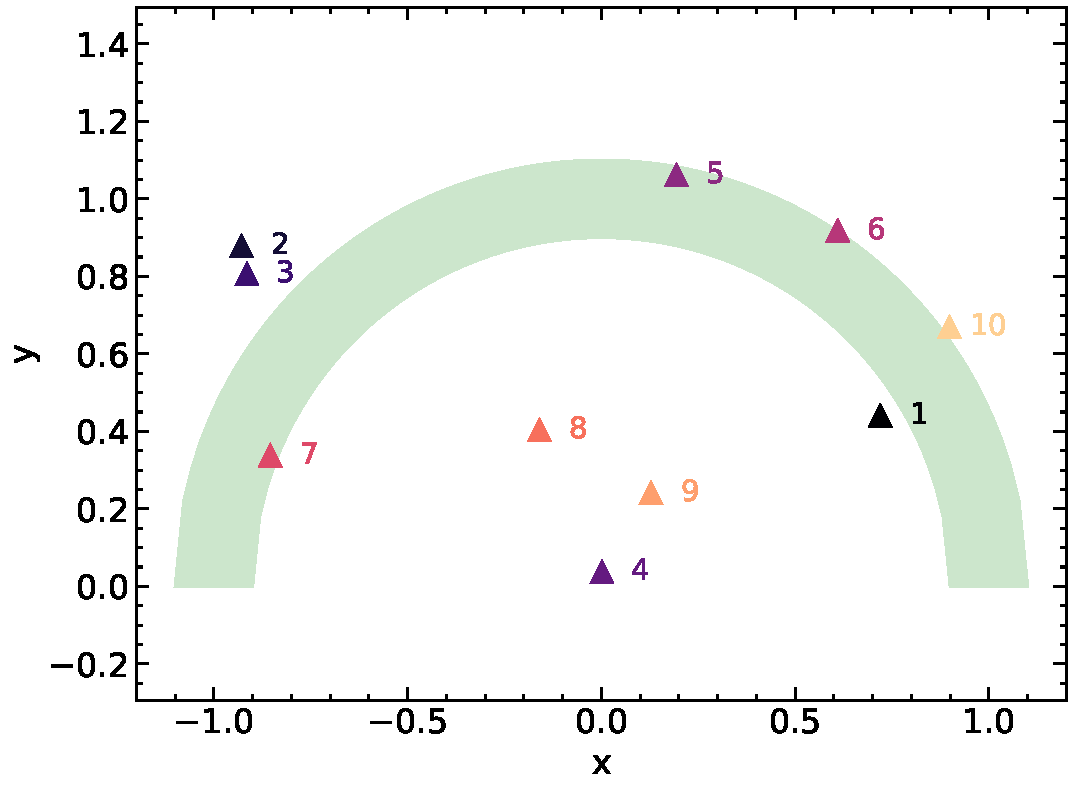
\includegraphics[width=0.5\textwidth]{figures/cond_inicial.pdf}
    \caption{valores iniciales de los pesos sinápticos de la red de Kohonen.}
    \label{fig:cond_inicial}
\end{figure}

\begin{figure*} [t]
    \centering
    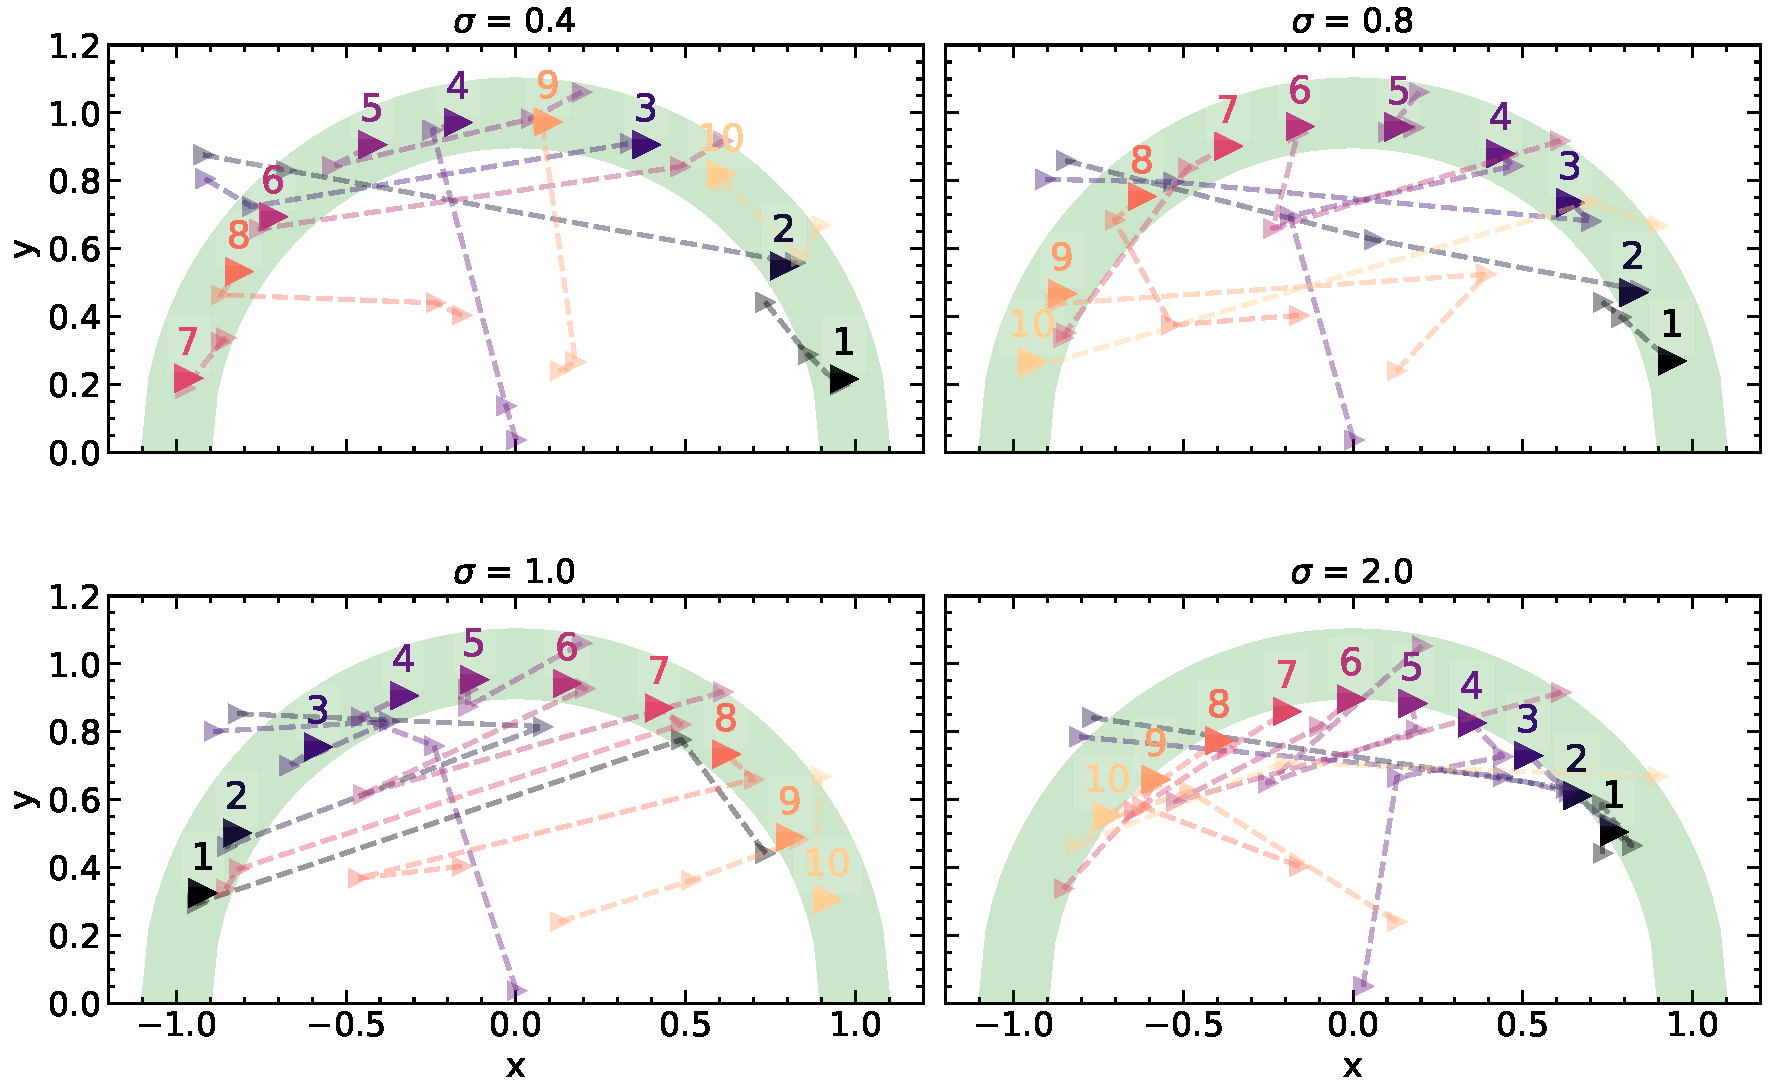
\includegraphics[width=\textwidth]{figures/ej_2_trainings.pdf}
    \caption{evolución en función de los ejemplos o iteraciones para diferentes valores de \(\sigma\). Se muestra la evolución con el número de ejemplos partiendo desde la semilla y las iteraciones correspondientes a \(10^2\), \(10^5\) y \(10^7\). Los colores muestran la salida analizada según la etiqueta de la figura.}
    \label{fig:ej2_pesos}

\end{figure*}

Como función de vecindad, se utilizó 

\begin{equation} \nonumber
    \Lambda(i, i^*) \propto  e^{-\frac{(i-i^*)^2}{2 \sigma^2}}
\end{equation}

\noindent donde i se corresponde i-ésima neurona (\(\omega_i\)), mientras que \(i^*\) es la neurona que se encuentra más cerca del valor de entrada.

Para realizar esta red, se utilizó una taza de aprendizaje de \(\eta = 0.1\) y se evaluaron diferentes valores de \(\sigma\) (0.4, 0.8, 1 y 2). Como la distancia entre los ``primeros vecinos'' es 1, un valor de \(\sigma < 1\) implica una menor corrección sobre los vecinos, mientras que un valor de \(\sigma \geq  1\) corrige sobre los vecinos, siendo mayor los vecinos afectados mientras mayor sea el valor de \(\sigma\).

Los resultados obtenidos para \(10^7\) ejemplos, así como la evolución en función de los ejemplos o iteraciones se muestran en la Figura \ref{fig:ej2_pesos}.

En la Figura \ref{fig:ej2_pesos} se observa que para \(\sigma = 0.4\) la red no logra ordenar de manera correcta las salidas ya que los vecinos se encuentran separador por \(\sim 2\sigma\), por lo que la función de vecindad tiende a 0. Para \(\sigma = 0.8\) se observa que la red logra ordenar de manera correcta las salidas, sin embargo, la convergencia es más lenta que para \(\sigma = 1\). Para \(\sigma = 2\) se observa que la red logra ordenar de manera correcta las salidas, pero las salidas se agrupan en el centroide del dominio. Además, lo que se nota es que para \(\sigma = 1\), el orden es contrario a los casos anteriores. Esto depende de como el algoritmo modifica los pesos según la cercanía según el \(\sigma\) dado, pero lo importante es que estén ordenados ya sea en una dirección u otra.

\end{document}